\documentclass{article}

\usepackage [utf8]{inputenc}
\usepackage[babel]{csquotes}
\usepackage [italian,english]{babel}					%Lingua e sillabazione
%\usepackage [english]{babel}
\usepackage {graphicx}									%Immagini
\usepackage {subfigure}
\usepackage {caption}									%Didascalie
\usepackage {wrapfig}									%Testo che avvolge un'oggetto
\usepackage {amsfonts, amsmath, amssymb, esint, mathrsfs}	%Font e simboli matematici
\usepackage {amsthm}										%Definizioni e teoremi
\usepackage {mathtools}									%Comandi abs e norm	definiti sotto
\usepackage {fancyhdr}									%Abstract in {book}
\usepackage {hyperref}									%Collegamenti rossi e verdi
\usepackage{braket}										%generate bra and ket vectors
\usepackage{bm}
\usepackage{bbm}

\usepackage[a4paper,left=3cm,right=3cm]{geometry}

% if you use this label name will show near by table and figure
%\usepackage {showlabels}

%should remove warning for textbraceleft
\usepackage[T1]{fontenc}

%Tabelle
\usepackage {booktabs}									
\usepackage {multirow}

%Per il typesetting di formule chimiche - comando \ce{formula}
%\usepackage {mhchem}	
										
%\usepackage {siunitx}

%Bib
\usepackage[citestyle=alphabetic,
            bibstyle=alphabetic,
            maxcitenames=1,
            hyperref,
            isbn=false,
            url=false,
            doi=false,
            eprint=false,
            firstinits=true,
            backend=biber]{biblatex}


% ti permette di usare \begin(comment) \end(comment)
\usepackage{verbatim}

%%%%%%%%%%%% Font Alternativi, a gruppi %%%%%%%%%%%%%%%%%%%
% \usepackage{mathpazo}
% \usepackage[scaled=.95]{helvet}
% \usepackage{courier}

% \usepackage{mathptmx}
% \usepackage[scaled=.90]{helvet}
% \usepackage{courier}

%\usepackage{fourier}

\newcommand{\mail}[1]{\href{mailto:#1}{\texttt{#1}}}

\usepackage {listings}						%Per il codice
	\lstset {
		language=C++,
%		inputencoding=utf8x,
%		frame=single,
		numbers=none,
		extendedchars=\true,
		showstringspaces=\false,
		basicstyle=\small,
		%Voglio i colori come li fa gedit!!
		keywordstyle=\color{darkgreen}\bfseries,
		commentstyle=\color{blue},
		stringstyle=\color{fuxia},
	}

\usepackage {color}							%Definire colori
	\ifx\color@rgb\@undefined\else
		\definecolor{darkgreen}{rgb}{0,0.55,0}
		\definecolor{fuxia}{rgb}{1,0,0.98}
	\fi



\makeatletter								%Gestione dei bookmark nel pdf
\newcommand\deftoclevel[2][chapter]{%
\expandafter\renewcommand\csname toclevel@#1\endcsname{#2}}
\makeatother		%il comando \deftoclevel{-1} riporta il bookmark fuori di un livello

% \usepackage {fancyhdr}						%Testatine ed Abstract in {book} come nella tesi liceo
% \fancyhf{}
% \fancyhead[RO,LE]{\thepage}
% \fancyhead[LO]{\nouppercase{\slshape\rightmark}}
% \fancyhead[RE]{\nouppercase{\slshape\leftmark}}
% \pagestyle{fancy}

\renewcommand{\epsilon}{\varepsilon}		%Definizione delle lettere greche per la tipografia italiana
\renewcommand{\theta}{\vartheta}
%\renewcommand{\rho}{\varrho}
\renewcommand{\phi}{\varphi}

\DeclareMathOperator{\NN}{\mathbb{N}}
\DeclareMathOperator{\RR}{\mathbb{R}}
\DeclareMathOperator\grad{grad}
\DeclareMathOperator\rot{rot}	
\DeclareMathOperator\curl{curl}	
\DeclareMathOperator\sym{sym}	
\DeclareMathOperator\tr{tr}	
\DeclareMathOperator\divergence{div}
\renewcommand{\div}{\divergence}
\DeclareMathOperator{\argmin}{arg\,min}

\theoremstyle{plain}
\newtheorem{lemma}{Lemma}
\theoremstyle{remark}
\newtheorem{osservazione}{Osservazione}
\theoremstyle{plain}
\newtheorem{teorema}{Teorema}
\theoremstyle{definition}
\newtheorem{algoritmo}{Algoritmo}

\DeclarePairedDelimiter{\abs}{\lvert}{\rvert}
\DeclarePairedDelimiter{\norma}{\lVert}{\rVert}

\def\d{\,\,\textrm{d}}				%il differenziale in testo dritto


%\def\wto{\overset{w}{\to}}
\def\wto{\rightharpoonup}
\def\vec{\mathbf}

\relpenalty=9999				%evita che le formule inline siano spezzate da fineriga QUASI sempre
\binoppenalty=9999				%impostare a 10000 per evitare SEMPRE

\newcommand{\<}{\langle}
\renewcommand{\>}{\rangle}

\newcommand{\numberset}{\mathbb}
\newcommand{\N}{\numberset{N}}
\newcommand{\R}{\numberset{R}}
\newcommand{\Z}{\numberset{Z}}

%Dichiarazione di teoremi e definizioni
\theoremstyle{definition}					
\newtheorem{definizione}{Definizione}

\theoremstyle{plain}
\newtheorem*{teorema_bis} {Teorema}
\newtheorem{proposizione}{Proposizione}

%%Bibliography
\bibliography{../src/library}
%\addbibresource{src/library.bib}

\usepackage{frontespizio}

\begin{document}
  
  %\frontmatter
  \begin{titlepage}
    
\begin{frontespizio}

\Istituzione{POLITECNICO DI MILANO}
\Logo{img/polimiLogo}
\Facolta{Ingegneria Industriale e dell'informazione}
\Corso[Laurea]{Ingegneria Matematica}
\Annoaccademico{2015-2016}
\Sottotitolo{ sottotitolo}
\Titolo{\color[rgb]{.6,0,0} Strategie e analisi dell'errore per problemi di ottimizzazione vincolati regolati da equazioni di evoluzione}
\Candidato[]{Claudia Bonomi matr. 804378}
\Candidato[]{Edoardo Arbib matr. }
\Titoletto{Progetto per il corso di Analisi Numerica per le Equazioni a Derivate Parziali II}
\Relatore{ Simona Perotto}
\Relatore{ Ilario Mazzieri}
\Rientro{1cm}
\Margini{1.5cm}{2cm}{1.5cm}{3cm}

\end{frontespizio}
  \end{titlepage}
%    \input{src/quotes}
%    \newcommand {\fncyblank}{\fancyhf{}}

\newenvironment {abstract}%
{%\fncyblank 
\null \vfill \begin {center}%
\bfseries \abstractname \end {center}}%



\begin{abstract}

\end{abstract}

\clearpage


%\begin{otherlanguage}{italian}
%  \begin{abstract}
%    Questo e` un lavoro figo.
%  \end{abstract}
%\end{otherlanguage}

%\fancyhf{}
%\fancyhead[RO,LE]{\thepage}
%\fancyhead[LO]{\nouppercase{\slshape\rightmark}}
%\fancyhead[RE]{\nouppercase{\slshape\leftmark}}
%\pagestyle{fancy}

%   \input{src/acknowledgments}
%    \chapter*{Nomenclature and Acronyms}

\subsubsection{A}

\begin{tabular}{l l l l}
\end{tabular}

\subsubsection{B}

\begin{tabular}{l l l l}
\end{tabular}

\subsubsection{C}

\begin{tabular}{l l l l}
\end{tabular}

\subsubsection{D}

\begin{tabular}{l l l l}
\end{tabular}

\subsubsection{E}

\begin{tabular}{l l l l}
\end{tabular}

\subsubsection{F}

\begin{tabular}{l l l l}
\end{tabular}

\subsubsection{G}

\begin{tabular}{l l l l}
\end{tabular}

\subsubsection{H}

\begin{tabular}{l l l l}
\end{tabular}

\subsubsection{I}

\begin{tabular}{l l l l}
\end{tabular}

\subsubsection{J}

\begin{tabular}{l l l l}
\end{tabular}

\subsubsection{K}

\begin{tabular}{l l l l}
\end{tabular}

\subsubsection{L}

\begin{tabular}{l l l l}
\end{tabular}

\subsubsection{M}

\begin{tabular}{l l l l}
\end{tabular}

\subsubsection{N}

\begin{tabular}{l l l l}
\end{tabular}

\subsubsection{O}

\begin{tabular}{l l l l}
\end{tabular}

\subsubsection{P}

\begin{tabular}{l l l l}
\end{tabular}

\subsubsection{Q}

\begin{tabular}{l l l l}
\end{tabular}

\subsubsection{R}

\begin{tabular}{l l l l}
\end{tabular}

\subsubsection{S}

\begin{tabular}{l l l l}
\end{tabular}

\subsubsection{T}

\begin{tabular}{l l l l}
\end{tabular}

\subsubsection{U}

\begin{tabular}{l l l l}
\end{tabular}

\subsubsection{V}

\begin{tabular}{l l l l}
\end{tabular}

\subsubsection{W}

\begin{tabular}{l l l l}
\end{tabular}

\subsubsection{X}

\begin{tabular}{l l l l}
\end{tabular}

\subsubsection{Y}

\begin{tabular}{l l l l}
\end{tabular}

\subsubsection{Z}

\begin{tabular}{l l l l}
\end{tabular}
%    \subsubsection{\textbf{Greek Symbols}}


\subsubsection{$ \mu $}

\begin{tabular}{l l l l}
\end{tabular}

\subsubsection{$ \nu $}

\begin{tabular}{l l l l}
\end{tabular}


\subsubsection{$ \Omega $}

\begin{tabular}{l l l l}
\end{tabular}
  \tableofcontents
  \newpage
  %\mainmatter
    \chapter{Introduzione}

Il lavoro qui presentato tratta lo studio di un problema di controllo ottimo parabolico attraverso l'analisi proposta da \cite{MAIN}.
\par\medskip
Per l'equazione di stato in tempo viene utilizzato uno schema Petrov-Galerkin con un approccio costante a tratti per la funzione di stato ed uno lineare a tratti per la funzione test. Questa scelta degli spazi funzionali ha una ripercussione sullo schema di discretizzazione temporale sia del problema di stato che del problema aggiunto. Per entrambi, infatti, sarà utilizzata una variante dello schema di Crank-Nicolson consistente con la teoria di Rannacher descritta in \cite{Ran84}.
In \cite{MAIN} viene provato analaticamente che questa scelta permette di raggiungere un ordine due di convergenza temporale sia per l'errore di controllo che per l'errore dello stato proiettato sulla griglia duale.
Per la discretizazione spaziale si è fatto riferimento all'analisi proposta in \cite{MV11}.
\par\medskip
Attraverso l'utilizzo del software \textbf{FreeFem++} l'approccio teorico proposto precedentemente è stato implementato. I risultati numerici ottenuti confermano quelli teorici e sono consistenti con quelli presentati in \cite{MAIN}. Per il calcolo dell'errore di controllo è stato utilizzato inizialmente il metodo di Cavalieri-Simpson. In seguito è stato calcolato un secondo algoritmo meno soggetto agli errori di approssimazione, con esso si trova unordine di convergenza maggiore di 2 per l'errore di controllo.
\par\medskip
Il report è strutturato nel seguente modo. Nel Capitolo \ref{chap:Continuos} viene analizzata la soluzione teorica del problema di controllo ottimo. Nel Capitolo \ref{chap:Discontinuos} viene analizzata la regolità del problema discontinuo e introdotte la semi-discretizzazione temporale e la discretizzazione spaziale. Nel Capitolo \ref{chap:Code} sono contenute le informazioni riguardanti l'implementazione dell'algoritmo. Nel Capitolo \ref{chap:Results} sono raccolti i risultati numerici. Nel Capitolo \ref{chap:Conclusion} sono contenute le conclusioni e spunti per lavori futuri.
    \chapter{Analisi del problema continuo}
\label{chap:Continuos}

Introdotto l'intervallo temporale $I = (0,T) \subset \mathbb{R}$, $T < \infty$ e una funzione scelta $y_d \in L^2(I,L^2)$ consideriamo dunque il seguente problema di controllo ottimo lineare quadratico:
{\renewcommand\arraystretch{2}
\begin{equation}
\tag{$\mathbb{P}$}
\begin{aligned}
& \underset{y \in Y, u \in U_{ad}}{\text{min}}
& & J(y,u) = \frac{1}{2}{||y-y_d||^{2}}_{L^2(I,L^2(\Omega))} + \frac{\alpha}{2}{||u||^{2}}_U \\
& \text{s.t.} & &  y = S(Bu,y_0) \\
\label{eq:200}
\end{aligned}
\end{equation}
} %chiude \renewcommand\arraystretch{1.5}
Lo spazio dello stato Y è definito come:
\begin{equation}
Y = W(I) =  \left\{ v \in L^2(I, {H^0}_1(\Omega)), {{\partial}_{t}}v \in L^2(I, H^{-1}(\Omega)) \right\}
\label{eq:201}
\end{equation}
dove
\begin{equation}
Y \hookrightarrow C(\left[0,T\right], L^2(\Omega))
\label{eq:202}
\end{equation}
    \chapter{Analisi del problema discreto}
\label{chap:Discontinuos}

\section{Semidiscretizzazione temporale}

\subsection{Caratteristiche dello schema numerico}
La sezione inizia introducendo la griglia e gli spazi funzionali utilizzati per la semidiscretizzazione temporale dei problemi di stato e aggiunto.

Si partizioni l'intervallo $[0,T)$ in sottointervalli $I_m=[t_{m-1},t_m)$, dove $0=t_0<t_1<\dots<t_M=T$ sono punti appartenenti al segmento $[0,T)$. Inoltre si affianchi a tale griglia una seconda partizione dell'intervallo $[0,T)$, fondamentale per ottenere i risultati di convergenza dei problemi semidiscretizzati, detta \textit{griglia duale}; essa è composta dagli intervalli $I^*_m=[t^*_{m-1},t^*_m)$, con $0=t^*_0<t^*_1<\dots<t^*_M=T$ e $t^*_m=\frac{t_{m-1}+t_m}{2}\quad\text{per $m=1,\dots,M$}$. Riassumendo si può contare su due suddivisioni dell'intervallo $[0,T)$ tali che $[0,T)=\bigcup^{M+1}_{m=1} I_m$ e $[0,T)=\bigcup^{M+1}_{m=1} I^*_m$.

Chiaramente la griglia primale avrà un parametro che ne descrive ``l'accuratezza'' che per noi sarà 
\[
k=\max_{1\le m\le M} k_m,\quad k_m=t_m-t_{m-1}\quad\text{per $m=1,\dots,M$}.
\] 

Per quanto riguarda l'ambientazione funzionale definiamo 
\begin{gather*}
P_k:=\Bigl\{v\in C([0,T],H^1_0(\Omega))\Bigl| v|_{I_{m}}\in \mathcal{P}_1(I_m,H^1_0(\Omega))\Bigr\}\hookrightarrow W(I),\\
P^*_k:=\Bigl\{v\in C([0,T],H^1_0(\Omega))\Bigl| v|_{I^*_{m}}\in \mathcal{P}_1(I^*_m,H^1_0(\Omega))\Bigr\}\hookrightarrow W(I),\\  
  Y_k:=\Bigl\{v:[0,T]\to H^1_0(\Omega)\Bigl| v|_{I_{m}}\in \mathcal{P}_0(I_m,H^1_0(\Omega))\Bigr\}\hookrightarrow W(I).
\end{gather*}
Qui, $\mathcal{P}_i(J,H^1_0(\Omega)), J\subset \overset{-}{I}, i\in\{0,1\}$, denota l'insieme dei polinomi in tempo al più di grado $i$ sull'intervallo $J$ a valori in $H^1_0(\Omega)$.


Nei risultati che si menzioneranno in seguito si farà spesso uso dei seguenti operatori di interpolazione:
\begin{enumerate}
\item $\mathcal{P}_{Y_{k}}:L^2(I,H^1_0(\Omega))\to Y_k$
\[
\mathcal{P}_{Y_{k}} v|_{I_{m}}:=\frac{1}{k_{m}} \int^{t_{m}}_{t_{m-1}}vdt\quad \text{for $m=1,\dots,M$},\quad\text{e}\quad \mathcal{P}_{Y_{k}}v(T):=0
\]
\item $\Pi_{Y_{k}}:C([0,T],H^1_0(\Omega))\to Y_k$
\[
\Pi_{Y_{k}} v|_{I_{m}}:=v(t^*_m)\quad\text{per $m=1,\dots,M$},\quad \Pi_{Y_{k}} v(T):=v(T)
\]
\item $\pi_{P^*_k}:C([0,T],H^1_0(\Omega))\cup Y_k\to P^*_k$
\begin{gather*}
\pi_{P^*_k} v|_{I^*_1\cup I^*_2}:=v(t^*_1)+\frac{t-t^*_1}{t^*_2-t^*_1}(v(t^*_2)-v(t^*_1)),\\
\pi_{P^*_k} v|_{I^*_m}:=v(t^*_{m-1})+\frac{t-t^*_{m-1}}{t^*_{m}-t^*_{m-1}}(v(t^*_m)-v(t^*_{m-1})),\quad\text{per $m=3,\dots,M-1$},\\
\pi_{P^*_k} v|_{I^*_M\cup I^*_{M+1}}:=v(t^*_{M-1})+\frac{t-t^*_{M-1}}{t^*_M-t^*_{M-1}}(v(t^*_M)-v(t^*_{M-1})).
\end{gather*}
\end{enumerate} 


\subsection{Semidiscretizzazione del problema di stato}
Uno degli elementi di novità del lavoro DHV è dato proprio dallo schema adottato per la discretizzazione in tempo dell'equazione di stato, che è totalmente variazionale di tipo Petrov-Galerkin. Verranno infatti utilizzati uno spazio di funzioni costanti a tratti per la soluzione e continue lineari a tratti per le test. 

Supponendo di estendere la forma bilineare $A$ di \cite{MAIN} in una mappa $A:W(I)\cup Y_k\times\to\R$, si tratta dunque di risolvere il seguente problema:

dati $(f,\kappa)\in L^2(I,H^{-1}(\Omega))\times L^2(\Omega)$, trovare $y_k\in Y_k$ tale che 
\begin{equation}
\label{eqn:stato}
A(y_k,v_k)=\int^{T}_{0} \Braket{f(t),v_k(t)}_{H^{-1}(\Omega)H^1_0(\Omega)}dt + (\kappa,v_k(0))_{L^2(\Omega)}\quad \forall v_k\in P_k.
\end{equation}
Data la scelta dello spazio $Y_k$ per la soluzione, essa può essere espressa come 
\[
y_k=\alpha_{M+1}\chi_{\{T\}} + \sum^M_{i=1} \alpha_i\chi_{I_i},\quad \alpha_i\in H^1_0(\Omega)\quad\text{per $i=1,\dots,M+1$},
\]
e attraverso facili calcoli si arriva alla formulazione del problema~\eqref{eqn:stato} in termini delle funzioni $\alpha_i$:
\begin{enumerate}
\item Trovare $\alpha_1$ tale che
\begin{equation}
\label{eqn:stato1}
\frac{1}{t_1-t_0}(\alpha_1-\kappa,g)_{L^2(\Omega)} + \frac{1}{2}a(\alpha_1,g)=\frac{1}{2}(f(0),g)_{L^2(\Omega)}\quad \forall g\in H^1_0(\Omega),
\end{equation}
\item Trovare $\alpha_i,i=2,\dots,M$ tale che 
\begin{equation}
\label{eqn:stato2}
 \frac{1}{t_i-t_{i-1}}(\alpha_i-\alpha_{i-1},g)_{L^2(\Omega)} + \frac{1}{2}a(\alpha_i+\alpha_{i+1},g)=\frac{1}{2}(f(t_{i-1}),g)_{L^2(\Omega)}\quad \forall g\in H^1_0(\Omega),
 \end{equation}
 \item Trovare $\alpha_{M+1}$ tale che 
\begin{equation}
\label{eqn:stato1}
\frac{1}{t_{M}-t_{M-1}}(\alpha_{M+1}-\alpha_M,g)_{L^2(\Omega)} + \frac{1}{2}a(\alpha_M,g)=\frac{1}{2}(f(t_{M}),g)_{L^2(\Omega)}\quad \forall g\in H^1_0(\Omega),
\end{equation}
\end{enumerate}
Alla luce di questa seconda formulazione si evince che lo schema di Petrov-Galerkin introdotto è equivalente ad una variante del metodo di Crank-Nicolson con primo e ultimo passo temporale di Rannacher, e sempre dalla seconda formulazione risulta chiaro che il problema semidiscretizzato ammette unica soluzione $y_k\in Y_k$.

A questo punto vengono enunciati senza dimostrazione alcuni risultati tratti da \cite{MAIN} che garantiscono la stabilità e convergenza del metodo di Petrov-Galerkin. Per la stabilità:
 \begin{lemma} 
 \label{stab:stato}
 Sia $y_k\in Y_k$ la soluzione di~\eqref{eqn:stato} con $f\in L^2(I,L^2(\Omega))$ e $\kappa\in L^2(\Omega)$ assegnati. Allora esiste una costante $C>0$ indipendente dal parametro di griglia $k$ tale che
 \[
 \norma{y_k}_I\le C(\norma{f}_I + \norma{\kappa}_{L^2(\Omega)})
 \]
\end{lemma}
 Passando ora all'analisi di convergenza è normale aspettarsi un'approssimazione di ordine $\mathcal{O}(k)$, poiché la $y_k$ é costante a tratti in tempo; tuttavia la proiezione di $y_k$ tramite l'operatore $\pi_{P^*_k}$ permette di ottenere stime di ordine $\mathcal{O}(k^2)$. Infatti,
 \begin{lemma} 
 \label{conv:stato}
 Siano $f\in H^1(I,L^2(\Omega)),f(0)\in H^1_0(\Omega)$ e $\kappa\in H^1_0(\Omega)$ con $\Delta\kappa\in H^1_0(\Omega)$ e siano $y,y_k$ le soluzioni dei problemi \ref{eq:201} e~\eqref{eqn:stato} con dati $(f,\kappa)$. Allora vale
 \[
 \norma{\pi_{P^*_k}y_k-y}_I\le Ck^2(\norma{\partial^2_t y}_I + \norma{\partial^2_t \Delta y}_I)
 \]
 \end{lemma}

\subsection{Semidiscretizzazione del problema aggiunto}
Anche il problema aggiunto viene affrontato con uno schema in tempo di tipo Petrov-Galerkin, dove però vengono scambiati gli spazi funzionali delle soluzioni e delle test. Poiché tale scelta conduce ad un metodo di Crank-Nicolson all'indietro, la sua analisi è standard. Si riportano qui di seguito la formulazione e risultati principali.

Problema aggiunto semidiscretizzato in tempo:

Dato $h\in L^2(I,H^{-1}(\Omega))$ trovare $p_k\in P_k$ tale che 
\begin{equation}
\label{eqn:agg}
A(\tilde{y},p_k)=\int^T_0 \Braket{h(t),\tilde{y}(t)}_{H^{-1}(\Omega)H^1_0(\Omega)}dt\quad\forall\tilde{y}\in Y_k
\end{equation}
Se si scrive $p_k$ nella forma 
\[
p_k(t)=\sum^M_{i=0}\beta_i b_i(t)
\]
con coefficienti $\beta_i\in H^1_0(\Omega)$ e $b_i\in C([0,T]), b_i(t_j)=\delta_{ij}$ per $i,j=0,\dots,M$, l'equazione~\eqref{eqn:agg} diventa equivalente a
\begin{enumerate}
\item $\beta_M=0$,
\item trovare $\beta_i,i=0,\dots,M-1$ tale che
\begin{equation}
\label{eqn:agg1}
\frac{1}{t_{i+1}-t_i}(\beta_i-\beta_{i+1},g)_{L^2(\Omega)} + \frac{1}{2}a(\beta_i+\beta_{i+1},g)=\frac{1}{2}(h(t_i)+h(t_{i+1}),g)_{L^2(\Omega)}\quad\forall g\in H^1_0(\Omega)
\end{equation}
\end{enumerate}
Stabilità e convergenza:
\begin{lemma}
\label{stab:agg}
Sia $p_k\in P_k$ la soluzione di~\eqref{eqn:agg} con $h\in L^2(I,L^2(\Omega))$. Allora esiste ina costante $C>0$ indipendente da $k$ tale che
\[
\norma{p_k}_{H^1(I,L^2(\Omega))} + \norma{p_k(0)}_{H^1(\Omega)} \le C\norma{h}_I.
\]
\end{lemma}
\begin{lemma}
\label{conv:agg}
Sian0 $p,p_k$ le soluzioni di \ref{eq:217} e di~\eqref{eqn:agg} rispettivamente, con $h\in L^2(I,L^2(\Omega))$. Allora vale
\[
\norma{p_k-p}_I\le Ck^2(\norma{\partial^2_t p}_I + \norma{\partial_t\Delta p}_I).
\]
\end{lemma}
    \chapter{Discretizzazione variazionale}
\label{chap:DiscVar}
Per approssimare il problema di controllo ottimo [P] viene applicato un metodo detto di discretizzazione variazionale, introdotto da M. Hinze in [Hin05]. Nella prossima sezione viene brevemente presentato questo metodo nel caso generale di problemi di controllo quadratici, dopodiché lo si vedrà in azione per  la risoluzione di \ref{eq:200}.   


\subsection{Il caso generale}

Si consideri il seguente problema di controllo ottimo quadratico
\begin{equation}
\label{controlpb}
\min_{(y,u)\in Y\times U} J(y,u)   \ \text{s.t.} \ y=Su \  \text{and} \ u\in U_{ad},
\end{equation}
dove $ U=U^*$ denota lo spazio di Hilbert del controllo, $ Y $ lo spazio di Banach dello stato, $ S:U\to Y\subseteq U $ l'operatore lineare e limitato tra controllo e stato, e $ U_{ad}\subseteq U $ l'insieme chiuso e convesso dei controlli ammissibili. Inoltre per $ \alpha>0 $ sia il funzionale $ J $ dato da 
\begin{equation}
J(y,u)=\frac{1}{2}\norma{y-z}^2_Z + \frac{\alpha}{2}\norma{u}^2_U,
\end{equation}
dove $ Z=Z^* $ denota uno spazio di Hilbert, $ z\in Z $ e $ Y\hookrightarrow Z\hookrightarrow Y^* $.   

La presente  discretizzazione di ~\eqref{controlpb} si basa sulla discretizzazione dei soli spazi di stato e aggiunto, utilizzando implicitamente le condizioni di ottimalità del primo ordine per la discretizzazione del controllo. Tra i vantaggi di tale approccio si consideri , nel caso si utilizzino schemi ad elementi finiti,  il disaccoppiamento dell'approssimazione dell'\textit{active set} dai nodi della griglia per gli EF. 

Per definire il controllo discreto sia $ S_h:U\to Y_h\subset Y\subseteq U$ l'operatore lineare limitato tra il controllo e lo stato discretizzato, dove $ Y_h\subseteq Y $ è uno sottospazio finito-dimensionale equipaggiato con la norma di $ Y $.
\begin{definizione}

$ u^*_h\in U_{ad} $ è detto controllo discreto ottimale $ \iff $
\begin{equation}
\label{contrpbdisc}
\big( \hat{J}'_h(u^*_h),v-u^*_h\big)_U \ge 0 \ \forall v\in U_{ad},
\end{equation}
dove $ \hat{J}'_h(u):=J(S_h u,u) $.
\end{definizione}
\begin{osservazione}

Nel caso di problemi di controllo quadratici vincolati (come per il presente lavoro) la disuguaglianza variazionale ~\eqref{contrpbdisc} è condizione di ottimalità necessaria e sufficiente di 
\begin{equation}
u^{*}_{h}= \argmin_{u \in U_{ad}} J(S_hu,u).
\end{equation}

\end{osservazione}.
Se esprimiamo la condizione di ottimalità ~\eqref{contrpbdisc} qualora $ U_{ad}=U $ appare chiaro come sia possibile realizzare uno schema numerico per risolvere un problema di ottimizzazione senza discretizzare lo spazio di controllo:
\begin{equation}
u^*_h=\frac{-1}{\alpha}S^*_h(S_hu^*_h-z),
\end{equation}
Infatti, sebbene $ u^*_h $ sia in $ U $, esso è implicitamente un oggetto discreto per via dell'operatore aggiunto discreto.

Ora si riporta senza dimostrazione il risultato principale legato alla discretizzazione variazionale, che poi sarà utile in seguito: 
\begin{teorema}
\label{teo:Hin}

Se gli operatori $ S_h, S^*_h $ soddisfano le condizioni
\begin{itemize}

\item $ \norma{(S^*-S^*_h)z}_U\le Ch^2\norma{z}_Z $
\item $ \norma{(S^*S-S^*_hS_h)u^*}_U\le Ch^2\norma{u^*}_U $

\end{itemize}
allora per $ h>0 $ sufficientemente piccolo la disuguaglianza variazionale ~\eqref{contrpbdisc} ammette un'unica soluzione $ u^*_h\in U_{ad} $ che soddisfa 
\begin{equation}
\norma{u^*-u^*_h}_U\le Ch^2\{ \norma{u^*}_U + \norma{z}_Z\}.
\end{equation}
Qui, $ u^*\in U_{ad} $ denota l'unica soluzione del problema ~\eqref{controlpb}.

\end{teorema}

\subsection{Il caso in oggetto}

Ora si vuole applicare il metodo di discretizzazione variazionale al problema [RIF] nei confronti della variabile tempo, dove gli operatori $ S_h $ e $ S^*_h $ sono individuati dagli schemi di Petrov-Galerkin esposti nei capitoli precedenti.

Dunque, il problema (semi)discretizzato da considerare è
\begin{gather}
\label{Pk}
\min_{y_k\in Y_k, u\in U_{ad}} J(y_k,u)=\frac{1}{2}\norma{y_k-y_d}^2_{L^2(I,L^2(\Omega))} + \frac{\alpha}{2}\norma{u}^2_U, \\
\text{s.t.} \ y_k=S_k(Bu,y_0),
\end{gather}
dove $ S_k $ è l'operatore delle soluzioni associato a [RIF]. Grazie ai risultati della precedente sezione questo problema ammette un'unica soluzione $ (\bar{y}_k, \bar{u}_k)\in Y_k\times U_{ad} $, con $ \bar{y}_k=S_k(B\bar{u}_k,y_0) $ e la condizione di ottimalità del primo ordine recita
\begin{equation}
\label{cnott}
\bar{u}_k=P_{U_{ad}}\big( -\frac{1}{\alpha}B'\bar{p}_k\big),
\end{equation}
dove $ \bar{p}_k\in P_k $ denota la variabile aggiunta discreta, che è l'unica soluzione di [RIF] con $ h:=\bar{y}_k-y_d $.
A partire dalla formulazione del problema ~\eqref{P_k} è possibile ottenere delle stime di convergenza che somigliano alla stima standard ottenuta per problemi con discretizzazione variazionale. Per completezza vengono trascritti qui di seguito tali risultati.
\begin{teorema}
\label{convu}

Siano $ \bar{u} $ e $ \bar{u}_k $ le soluzioni di [RIF]  e di ~\eqref{Pk} rispettivamente. Allora
\begin{multline} 
\alpha \lvert \bar{u}_k-\bar{u}\rvert_I\le Ck^2\big( \norma{\bar{u}}_{H^1(I,\R^D)} + \norma{\bar{u}(0)}_{\R^D} + \\
\norma{y_d}_{H^1(I,L^2(\Omega))} + \norma{y_d(T)}_{H^1(\Omega)} + \norma{y_0}_{H^1(\Omega)} + \norma{\Delta y_0}_{H^1(\Omega)}\big)
\end{multline}
è soddisfatta.

\end{teorema}

\begin{teorema}
\label{convy}

Siano $ \bar{u} $ e $ \bar{u}_k $ le soluzioni di [RIF] e~\eqref{Pk} rispettivamente. Allora vale
\begin{multline}
\norma{\bar{y}-\pi_{P^*_k}\bar{y_k}}_I\le\big( \lvert a\rvert_I + \norma{\bar{u}}_{H^1(I,\R^D)} + \norma{\bar{u}(0)}_{\R^D} + \\ 
\norma{y_d}_{H^1(I,L^2(\Omega))} + \norma{y_d(T)}_{H^1(\Omega)} + \norma{y_0}_{H^1(\Omega)} + \norma{\Delta y_0}_{H^1(\Omega)}\big).
\end{multline}

\end{teorema}  

\section{Metodo di punto fisso}

L'equazione ~\eqref{cnott} è incline ad essere risolta numericamente nonostante il controllo non sia discretizzato esplicitamente; nel presente lavoro vengono scelti schemi di punto fisso e Newton con damping (semi-Newton).

Per quanto riguarda il metodo di punto fisso, se si indica con $ S^*_h $ l'operatore di soluzione dell'equazione [RIF], l'algoritmo è il seguente:
\begin{algoritmo}

\begin{enumerate}
\item Inizializzare $ u^0_h\in U_{ad} $, $ n:=0 $.
\item Ripetere fino a convergenza
          \begin{enumerate}
          \item calcolare $ Bu^n_h $,
          \item calcolare $ y^n_h=S_h(y_0,Bu^n_h) $, 
          \item calcolare $ p^n_h=S^*_h(y^n_h-y_d) $,
          \item calcolare $ u^{n+1}_h=P_{U_{ad}}\big( -\frac{1}{\alpha}B'p^n_h\big) $,
          \item porre n=n+1.
          \end{enumerate}
\end{enumerate}

Come criterio di arresto è stato scelto   
\begin{equation}
\norma{B'\big(p^{n+1}_h-p^n_h\big)}_{L^{\infty}(\Omega\times I)}<\epsilon,
\label{eq:PuntoFissotoll}
\end{equation}
con $ \epsilon $ tolleranza prefissata.
\label{PuntoFisso}
\end{algoritmo}

Seguendo [RIF] il metodo di punto fisso per l'equazione ~\eqref{cnott} converge globalmente per $ \alpha>\norma{S_h}^2_{\mathcal{L}(L^2(\Omega),L^2(\Omega))} $, motivo per cui è stato implementato anche lo schema semi-Newton, che ha invece la pretesa di convergere globalmente per qualsiasi valore di $ \alpha $.

    \lstnewenvironment{Code}[1][]{\lstset{basicstyle=\small\ttfamily, columns=fullflexible,framexrightmargin=+.1\textwidth, keywordstyle=\color{red}\bfseries, commentstyle=\color{blue},language=C++, basicstyle=\small, numbers=left, numberstyle=\tiny, stepnumber=1, numbersep=5pt, frame=shadowbox, #1}}{}

%\chapter{Descrizione Implementazione}
\section{Descrizione Implementazione}
\label{chap:Code}

In questo capitolo verranno descritte la struttura di base e le funzioni principali del codice sviluppato.
Per l'implementazione del codice si è utilizzato il solver \href{http://www.freefem.org/}\texttt{FreeFem$++$}\footnote{http://www.freefem.org/} ed il relativo linguaggio di programazione. Durante tutte le fasi di sviluppo del codice è stata utilizzata la piattaforma di hotsing web \href{https://github.com/}{\texttt{GitHub}}\footnote{https://github.com/}. Questo ha sia reso più fluida la collaborazione fra gli autori che garantito un maggiore controllo sull'avanzamento del codice.

\subsection{Strumenti di sviluppo}
\subsubsection{\texttt{FreeFem$++$}}
\href{http://www.freefem.org/}\texttt{FreeFem$++$} è un software per la risoluzione di equazioni alle derivate parziali che ha un proprio linguaggio di scripting basato sul C$++$. Gli script permettono di risolvere sistemi non lineari di più variabili in un dominio 2D o 3D.
\texttt{FreeFem$++$} è un software libero, disponibile per i sistemi operativi \textit{Linux}, \textit{Solaris}, \textit{OS X} and \textit{MS Windows}.

\subsubsection{\texttt{GitHub}}
{\texttt{Git}} è un sistema di controllo versione utilizzabile direttamente da linea di comando, molto diffuso e utile per tenere traccia delle varie fasi di sviluppo del codice. \texttt{GitHub} gestisce in modo adeguato i contributi al codice provenienti da agenti esterni e permette la condivisione del codice.\\
Il codice del progetto è reperibile su \texttt{GitHub} ed è possibile scaricarlo e collabolare allo sviluppo clonando il codice dalla repository  \href{https://github.com/}{\texttt{GitHub}}:\\
\begin{center}
\texttt{ git clone https://github.com/ClaB90/Progetto\_ANEDP}
\end{center}
Nella cartella principale è contenuto anche un file \texttt{.gitignore}, in cui sono specificate le estensioni dei files e le sottocartelle che non devono essere visionati in una repository \texttt{GitHub}. In particolare non si è interessati ai files temporanei che vengono eventualmente generati dagli editor.

\subsection{Implementazione}
In questo lavoro sia l'algoritmo \ref{PuntoFisso} di punto fisso che l'algoritmo \ref{DN} di Newton  sono stati implementati per la soluzione del problema parabolico di controllo ottimo \eqref{eq:200} descritto nei capitoli precedenti.
Il corpo del programma è costituito dal file \textbf{main.edp} che permette di risolve il problema \ref{Pk} con uno dei due algoritmi su una o più griglie temporali. Il processo di raffinamento temporale considera griglie, della tipologia introdotta nella sezione \ref{chap:Discontinuos}, uniformi tali che il numero di nodi Nk al livello l di infittimento sia:
\begin{equation}
Nk = ( 2^l + 1 )
\label{Nk}
\end{equation}
I valori della soluzione approssimata $u_k$ del problema di controllo vengono salvati per ogni livello di raffinamento in dei file di testo esterni per poter esser confrontati graficamente coi valori della soluzione esatta, nei casi in cui quest'ultima sia nota.
\par
L'errore fra la soluzione esatta e la soluzione approssimata per le funzioni di stato, aggiunta e controllo viene calcolato e salvato in un file di testo ad ogni livello. Questo permette il calcolo dell'ordine di convergenza per i diversi errori.
\par
Gli altri file principali sono i seguenti:
\begin{itemize}
\item[-] \texttt{controlparameters.edp}: contiene i parametri che definiscono il problema di controllo;
\item[-] \texttt{controlfunction.edp}: contiene le funzioni per l'algoritmo \ref{PuntoFisso} di punto fisso e per semi Newton \ref{DN};
\item[-] \texttt{UabSet.edp}: contiene i parametri limite dell'insieme $U_{ad}$ e le funzioni di proiezione per uno scalare e per un vettore sullo spazio $U_{ad}$;
\item[-] \texttt{funzioni.edp} contiene le funzioni che caratterizzano l'operatore B, la funzione yd e la forzante del problema di stato $g_0$, che verrà definita nella sezione \ref{chap:Results};
\item[-] \texttt{soluzioniEsatte.edp}: definisce le funzioni per le soluzioni esatte del problema di stato y, del problema aggiunto p e per la variabile di controllo u;
\item[-] \texttt{mesh.edp}: contine la definizione del dominio, la mesh ed il paramentro N di discretizazione spaziale;
\item[-] \texttt{state.edp}: in questo file viene definito il problema di stato. In particolare vengono introdotti lo spazio degli elementi finiti, la soluzione y0 all'istante iniziale, la definizione delle matrici di Stiffness e la funzione per la risoluzione del problema di stato;
\item[-] \texttt{adjoint.edp}: in questo file viene definito il problema aggiunto. Anche in questo caso vengono introdotti lo spazio degli elementi finiti, la soluzione pT all'istante finale, la definizione delle matrici di Stiffness e la funzione per la risoluzione del problema di aggiunto; 
\item[-] \texttt{normeeprodotti.edp}: contiene tutte le funzioni implementate per il calcolo delle norme e dei prodotti scalari; 
\item[-] \texttt{funzioniErrore.edp} e \texttt{funzioniErroreAdj.edp}: contengono le funzioni per il calcolo dell'errore delle variabili y,p e u;
\item[-] \texttt{funzioniCG.edp}: contiene le funzioni necessarie per l'algoritmo del gradiente coniugato \ref{CG}; 
\item[-] \texttt{saveme.edp} e \texttt{saveerr.edp}: descrivono le funzioni per salvare i valori della soluzione approsimata di controllo e dell'aggiunto e degli errori al termine dell'algoritmo per una data griglia temporale. Inoltre contiene la funzione per il calcolo dell'ordine di convergenza dell'errore in tempo;
\end{itemize}
Per il calcolo di ogni norma e prodotto scalare il metodo numerico di integrazione in tempo utilizzato è il metodo di Cavalieri Simpson. \MakeUppercase{è} stata fatta questa scelta poichè questa formula di Newton-Cotes ha un errore di quadratura sufficientemente basso da non influenzare l'analisi degli errori oggetto di studio.
\par
Per i problemi parabolici di controllo ottimo è necessario salvare matrici molto grandi contenenti le soluzioni del problema di stato e del problema aggiunto ad ogni istante temporale considerato. Questa richesta può portare a problemi di insufficiente memoria RAM durante l'esecuzione del programma. Tuttavia in questo lavoro non sono stati riscontrati problemi di questo tipo, e per una maggiore velocità di calcolo le soluzioni sono state tenute in memoria.
\subsubsection{Calcolo dell'errore}
Per il calcolo dell'errore della soluzione approssimata $u_k$ del problema di contollo particolare attenzione è stata posta sulla griglia di integrazione. La soluzione del problema aggiunto $p_k$ è una funzione continua lineare a tratti nel tempo i cui punti di non derivabilità coincidono con i nodi della griglia. La soluzione $u_k$, equazione \eqref{cnott}, è ancora una funzione funzione continua lineare a tratti nel tempo, ma l'operazione di proiezione $P_{U_{ab}}$ non garantisce che i nodi della griglia temporale utilizzata corrispondano a i punti di non derivabilità della funzione stessa, come mostrato in Figura \ref{fig:griglie}.
\begin{figure}
\centering
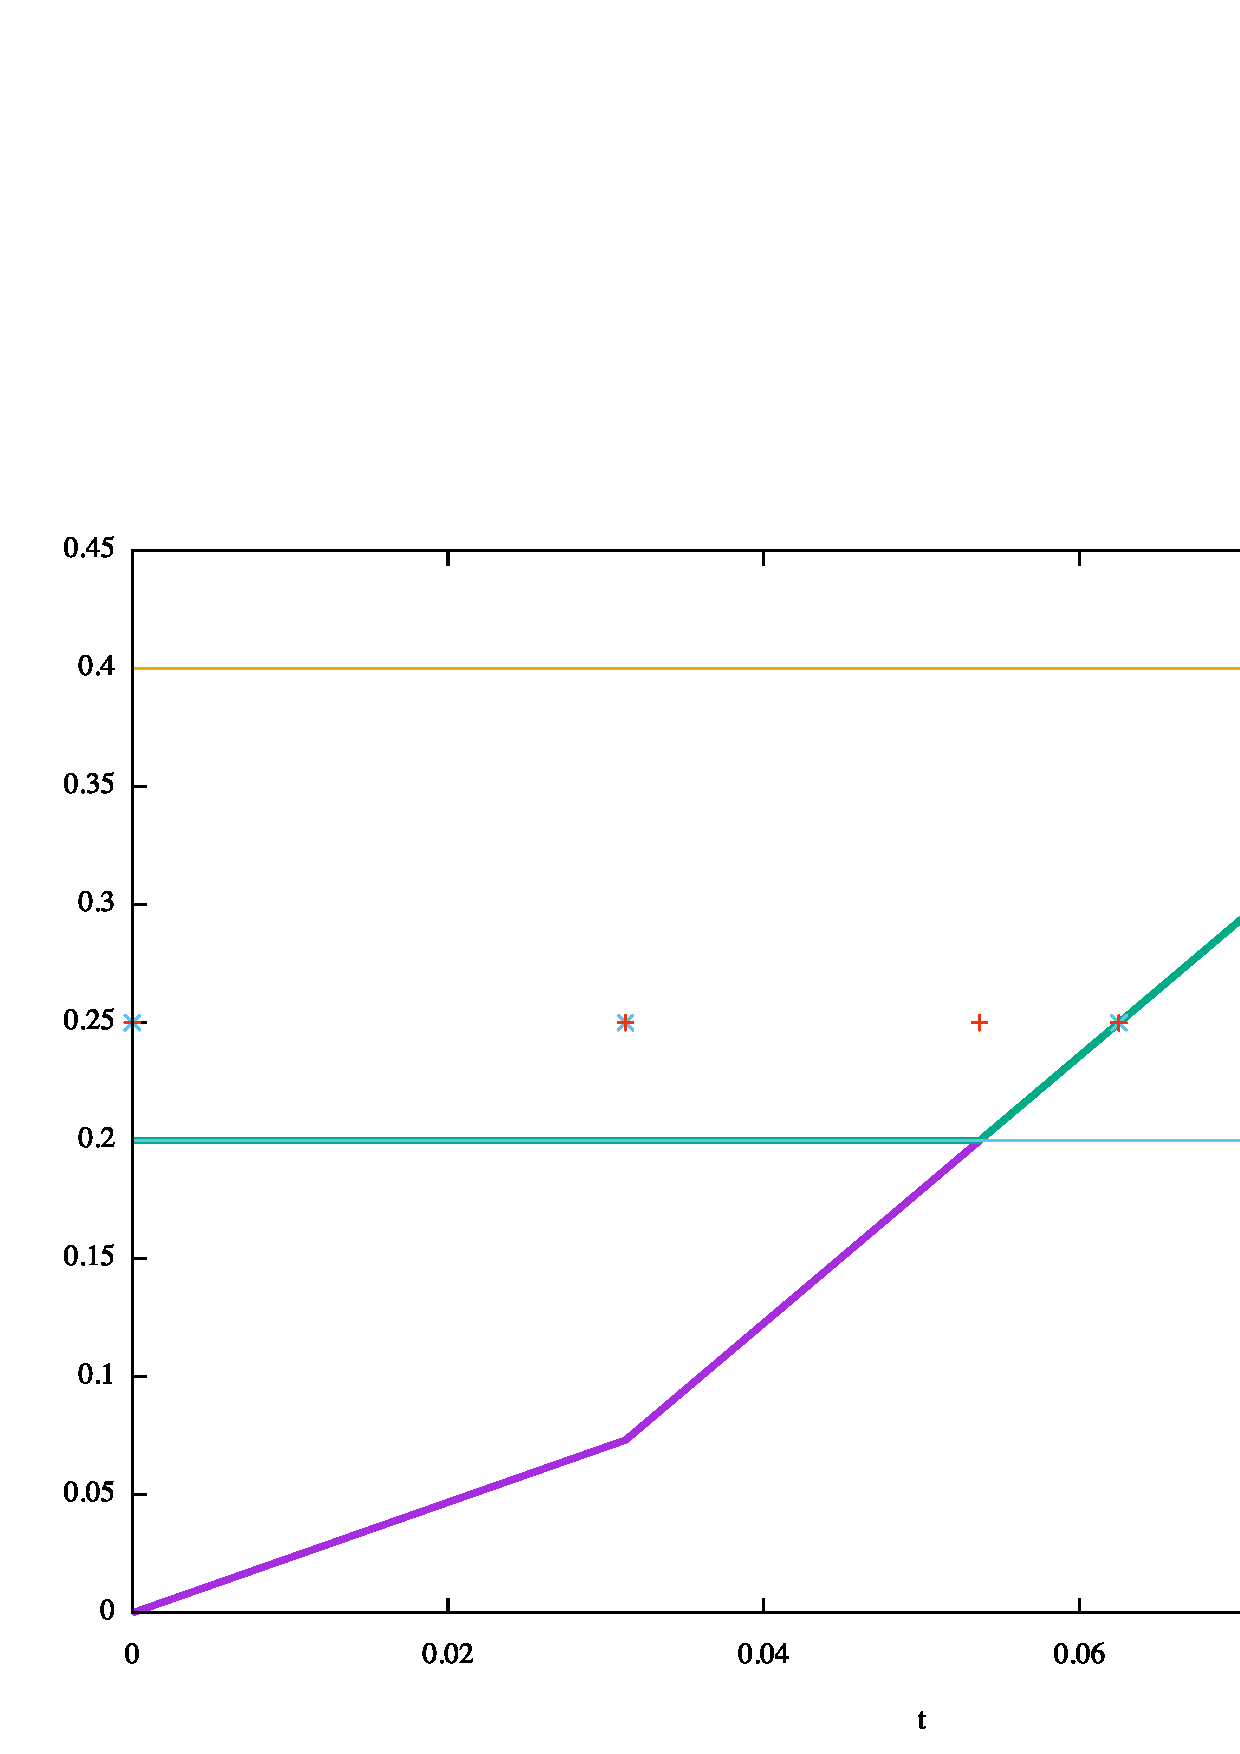
\includegraphics[scale=0.45]{img/cap5/griglie}
\caption{Esempio di differenza fra la griglia per la soluzione $u_k$ e la soluzione di $p_k$}
\label{fig:griglie}
\end{figure}
La funzione:
\begin{Code}[caption={Funzione \texttt{controlErrL2}}]
func real controlErrL2(real[int] &controlsol)
\end{Code}
Prende in ingresso la soluzione approssimata $u_k$ e calcola la norma $L^2(I,L^2(\Omega))$ della differenza con la soluzione esatta $\overline{u}$, equazione \eqref{eq:errcon},utilizzando il metodo di integrazione di Cavalieri-Simpson sulla griglia della soluzione $u_k$ invece che su quella generale. Anche in questo caso il motivo di questa scelta è quello di ridurre al minimo l'influenza degli errori di integrazione rispetto a quello dovuto all'approssimazione della soluzione.
\begin{equation}
err_{u_k} = || \overline{u} - u_k ||_{L^2(I,L^2(\Omega))}
\label{eq:errcon}
\end{equation}
\par
Per questo studio è di particolare interesse anche l'errore della soluzione di stato $y_k$ proiettata sullo spazio $P^*_k$ definito come:
\begin{equation}
err_{\pi_{P^*_k}y_k} = || \overline{y} - \pi_{P^*_k}y_k ||_{L^2(I,L^2(\Omega))}
\label{eq:errprojstate}
\end{equation}
dove $\overline{y}$ è la soluzione esatta del problema di stato e $\pi_{P^*_k}$ è definito nella sezione \ref{chap:Discontinuos}.
Il calcolo dell'errore \eqref{eq:errprojstate} è eseguito dalla funzione \texttt{stateprojtrap()}.
\par
La funzione \texttt{normL2state()}, invece, calcola l'errore per il problema di stato non proiettato definito da:
\begin{equation}
err_{y_k} = || \overline{y} - y_k ||_{L^2(I,L^2(\Omega))}
\label{eq:errstate}
\end{equation}
La funzione \texttt{normL2adj()} calcola infine l'errore per il problema aggiunto definito da:
\begin{equation}
err_{p_k} = || \overline{p} - p_k ||_{L^2(I,L^2(\Omega))}
\label{eq:erradj}
\end{equation}

\subsubsection{Punto Fisso}
Il primo procedimento implementato, di tipo Punto Fisso segue l'\textbf{Algoritmo} \ref{PuntoFisso}.
\par
Lo schema di integrazione temporale per il problema di stato è una variante dello schema di Crank-Nicolson(CN). In particolare viene effettuato un primo passo di Eulero all'indietro(EI) con parametro di griglia $\frac{{\Delta}t}{2}$, poi lo schema di Crank-Nicolson ed infine un passo di Eulero in avanti(EA).
\begin{Code}[caption={Funzione \texttt{setscheme()}}]
int setscheme(int value)
{
	// EI => value == 0
	if(value == 0)
	{
	    gamma1=1./2.;
	    gamma2=0.;
	    gamma3=0.;
	    gamma4=1./2.;
	}
	// CN => value == 1
	else if (value == 1)
	{	
		gamma1=1./2.;
	    gamma2=1./2.;
	    gamma3=0.;
	    gamma4=1.;
	}
	// EA => value == 2
	else if (value == 2)
	{
		gamma1=0.;
	    gamma2=1./2.;
	    gamma3=1./2.;
	    gamma4=0.;
	}
	
	return 0;
}
\end{Code}
Poichè la matrice di Stiffness rimane invariata fino al passo di Eulero in avanti per il problema di stato sono state definite due matrici:
\begin{Code}[caption={Matrici \texttt{s(w,wtest)} e \texttt{statetn(w,wtest)}}]
varf s(w,wtest) =   int2d(Th)( w*wtest/dt )
	        	  + int2d(Th)( gamma1*( dx(w)*dx(wtest) + dy(w)*dy(wtest) ) )
				  + on(1,2,3,4, w=wb);

varf statetn(w,wtest) =   int2d(Th)( wold*wtest/dt)
				  		- int2d(Th)( gamma2*(   dx(wold)*dx(wtest) 
				  							 + dy(wold)*dy(wtest) ) )
							//contributo di u
						+ int2d(Th)( gamma3*( g*ui*wtest ))
				 		+ int2d(Th)( gamma4*( g*uold*wtest ))
							//contributo di g0
						+ int2d(Th)( gamma3*( g0*wtest ))
				 		+ int2d(Th)( gamma4*( g0old*wtest ));
\end{Code}
In questo modo la matrice di Stiffness \texttt{s(w,wtest)} verrà calcolata solamente al primo ed all'ultimo passo dell'algoritmo, permettendo una riduzione del tempo di esecuzione. Il termine forzante $g_0$ verrà introdotto nella sezione \ref{chap:Results}.
\par
La funzione che calcola la soluzione $y_k$ ad ogni passo è \texttt{statet()} che prima di terminare calcola anche l'errore \eqref{eq:errprojstate} ed \eqref{eq:errstate}.
\par
Anche per il problema aggiunto è stato utilizzato un metodo di Crank-Nicolson ed è possibile trovare una matrice di Stiffness principale invariante nel tempo:
\begin{Code}[caption={Matrici \texttt{adj(w,wtest)} e \texttt{adjtn(w,wtest)}}]
varf adj(p,ptest) =   int2d(Th)( p*ptest/dt )			
					+ int2d(Th)( 0.5*( dx(p)*dx(ptest) + dy(p)*dy(ptest) ) ) 
				    + on(1,2,3,4, p=pb);

varf adjtn(p,ptest) =   int2d(Th)( pnext*ptest/dt )
    				  - int2d(Th)( 0.5*( dx(pnext)*dx(ptest) + dy(pnext)*dy(ptest) ) ) 
  					  + int2d(Th)( 0.5*( h*ptest ) ) 
  					  + int2d(Th)( 0.5*( hnext*ptest ) ); 
\end{Code}
dove \texttt{adj(p,ptest)} è invariante ad ogni passo temporale.
\par
Particolare attenzione è stata posta per il calcolo di h ed hnext che rapresentano il valore della forzante al passo i ed i+1. Per una corretta implementazione del metodo ad ogni passo i vale che:
\begin{equation}
h_i = {y_k}_i - y_d(t_i), \quad
hnext_i = {y_k}_i - y_d(t_i+{\Delta}t)
\label{hhnext}
\end{equation}
dove $t_i$ è il tempo considerato all'iterazione i-esima\footnote{Come si vede dalla formulazione debole \eqref{eqn:agg}}.
La funzione che calcola la soluzione $p_k$ ad ogni passo è la funzione \texttt{adjointt()} che prima di terminare valuta e salva l'errore per il problema aggiunto definito da \eqref{eq:erradj}. Inoltre in questa funzione vengono calcolati i valori della soluzione di controllo non proiettata:
\begin{equation}
{u_k}_i = -\frac{1}{\alpha}B'{p_k}_i  %= -\frac{1}{\alpha}*int2d(Th)( {p_k}_i * g ); 
\label{unp}
\end{equation}
\par
Infine la funzione \texttt{puntoFisso()} risolve l'\textbf{Algoritmo} \ref{PuntoFisso} rispettando il criterio di tolleranza \eqref{eq:PuntoFissotoll}.

\subsubsection{Semi-Newton}
Il secondo procedimento implementato, di tipo semi Newton, segue l'\textbf{Algoritmo} \ref{DN} e richiede l'ausilio del metodo del gradiente coniugato, \ref{CG}.
\par
Per la soluzione del problema di stato son state implementate due diverse funzioni. La prima chiamata \texttt{stateCG(real[int] \&xx)} risolve il problema di stato ad ogni passo temporale dato un termine noto e crea/restituisce il vettore delle soluzioni. L'operatore implementato è $S_h$ applicato a $P_{U_{ad}}(xx)$.
In particolare il termine noto, per una corretta proiezione sullo spazio $U_{ad}$, deve essere della forma:
\begin{equation}
xx = -\frac{1}{\alpha}*{S^{*}}_{h}(w)
\end{equation}
La seconda, denominata \texttt{mat1(real[int] \&xx, real[int] \&ww)}, risolve invece l'operatore $S_h\mathbbm{1}_{S^*_hw}$ applicato sempre a un termine noto xx. Questa operazione è necessaria per la costruzione di \eqref{newton}. Il vettore in ingresso ww contiene i valori dell'indicatrice $\mathbbm{1}_{S^*_hw}$.
L'algortimo seguito dalle queste funzioni è simile. Le differenze principali si trovano nella definizione del termine noto per il problema di stato. Nel primo caso verrà introdotta:
\begin{Code}[caption={Matrice \texttt{tnnew(w,wtest)} per \texttt{stateCG(real[int] \&xx)}}]
varf tnnew(w,wtest) =   int2d(Th)( wold*wtest/dt )
				  	  - int2d(Th)( gamma2*( dx(wold)*dx(wtest) + dy(wold)*dy(wtest) ) )
						//contributo di u
					  + int2d(Th)(gamma3*g*(PUabScal(listate)*wtest))
					  + int2d(Th)(gamma4*g*(PUabScal(loldstate)*wtest)) 
						//contributo di go 
					  + int2d(Th)( gamma3*( g0*wtest ))
			 		  + int2d(Th)( gamma4*( g0old*wtest ));
\end{Code}
dove le variabili \textit{listate} e \textit{listateold} rappresentano i valori dell'operazione di controllo dovuta al moltiplicatore di lagrange, mentre $g_0$ è il termine forzante.
\begin{Code}[caption={Matrice \texttt{tnnew(w,wtest)} per \texttt{mat1(real[int] \&xx, real[int] \&ww)}}]
varf tnnew(w,wtest) =  int2d(Th)( wold*wtest/dt) 
	  				 - int2d(Th)( gamma2*( dx(wold)*dx(wtest) + dy(wold)*dy(wtest) ) ) 
				     + int2d(Th)(gamma3*g*((indnew<=b)*(indnew>=a)*listate*wtest))
					 + int2d(Th)(gamma4*g*((indold<=b)*(indold>=a)*loldstate*wtest));
\end{Code}
dove le variabili \textit{listate}, \textit{listateold} rappresentano i valori dell'operazione di controllo dovuta al moltiplicatore di Lagrange, mentre \textit{indnew} ed \textit{indold} quelli dell'indicatrice $\mathbbm{1}_{S^*_hw}$.
In entrambe lo schema di integrazione temporale per il problema di stato segue la variante dello schema di Crank-Nicolson(CN) introdotta precedentemente per l'\textbf{Algoritmo} \ref{PuntoFisso} di punto fisso.
\par
La funzione \texttt{adjCG(real[int,int] \&xx)} implementa l'operatore $S^*_h$; risolve il problema aggiunto ad ogni passo temporale dato un termine noto xx e restituisce la soluzione in un opportuno vettore. Il procedimento utilizzato rispecchia quello precedentemente implementato per il metodo di punto fisso.
La funzione \texttt{CG(real[int,int] \&xx, real[int,int] \&ww)} risolve il sistema di equazioni \eqref{newton} tramite il metodo del gradiente coniugato introdotto in \ref{CG}. Ia matrice ww corrisponde al valore iniziale ${\delta}w^0$  mentre xx. CHIEDI EDO!
Infine la funzione \texttt{DampedNewton()} risolve l'\textbf{Algoritmo} \ref{DN} rispettando il criterio di tolleranza \eqref{eq:DNtoll}.
 	%\chapter{Risultati numerici}
\section{Risultati numerici}
\label{chap:Results}
In questo capitolo verranno esposti i risultati numerici ottenuti.
I primi due esampi sono stati presi da \cite{MAIN}.
In entrambi questi esempi verrà considerato l'operatore lineare affine $\tilde{B}$ \ref{eq:210}.

\subsection{Test Case 01}
\subsubsection{Set-up}
Il primo esempio considerato, in accordo con l'ipotesi i) introdotta in Chapter \ref{chap:Continuo}.
Preso il dominio spazio-temporale $\Omega \times I = (0,1)^2 x(0,0.01)$ e d=1, si considera l'operatore di controllo lineare affine $\tilde{B}$ che può essere completamente caratterizato da:
{\renewcommand\arraystretch{2}
\begin{equation}
\begin{array}{c}
g_1(t,x_1,x_2) = sin({\pi}x_1)sin({\pi}x_2)\\
g_0(t,x_1,x_2) = -{\pi}^2w_a(t,x_1,x_2) - BP_{U_{ad}} \left( -\frac{1}{4\alpha}(exp(a{\pi}^2t)-exp(a{\pi}^2T)) \right)
\end{array}
\label{eq:500}
\end{equation}
}
dove
\begin{equation}
w_a(t,x_1,x_2) = exp(a{\pi}^2t)sin({\pi}x_1)sin({\pi}x_2) \text{, } a \in \mathbb{R}
\label{eq:501}
\end{equation}
In particolare vengono considerate le costanti $a=-\sqrt{5}$ ed $\alpha={pi}^{-4}$.
Come conseguenza di ciò si ha che \ref{eq:212} verrà riscritta, utilizzando l'aggiunto di B e non $\tilde{B}$, come:
\begin{equation}
(B'z)(t) = \int_{\Omega} z(t,x_1,x_2)g_1(t,x_1,x_2) ,dx_1dx_2
\label{eq:502}
\end{equation}
Si definiscono ora:
{\renewcommand\arraystretch{2}
\begin{equation}
\begin{array}{c}
y_d(t,x_1,x_2) = \frac{a^2 - 5}{2 + a}{pi}^2w_a(t,x_1,x_2) + 2{pi}^2w_a(T,x_1,x_2) \\
y_0(x_1,x_2) = \frac{- 1}{2 + a}{pi}^2w_a(0,x_1,x_2)
\end{array}
\label{eq:503}
\end{equation}
}
L'insieme ammissibile $U_{ad}$ è limitato inferiormente da $a_1=-25$ e superiormente da $b_1=-1$.
Infine definiamo le soluzioni esatte per il problema di controllo ottimo \ref{eq:200}:
{\renewcommand\arraystretch{2}
\begin{equation}
\begin{array}{c}
\overline{u}(t,x_1,x_2) = P_{U_{ad}} \left( -\frac{1}{4\alpha}(exp(a{\pi}^2t)-exp(a{\pi}^2T)) \right) \\
\overline{y}(t,x_1,x_2) = \frac{- 1}{2 + a}{pi}^2w_a(0,x_1,x_2) \\
\overline{p}(t,x_1,x_2) = w_a(t,x_1,x_2) - w_a(T,x_1,x_2)
\end{array}
\label{eq:504}
\end{equation}
}

\subsubsection{Risultati Numerici}
\begin{figure}
\centering
\includegraphics[width=\linewidth]{img/cap6/TestCase01_ues_paper}
\caption{Test Case 01 $\overline{u}$ e $u_k$ risultati di \cite{MAIN}}
\label{fig:500}
\end{figure}

\begin{figure}
\centering%
\subfigure[\protect\url{l = 1}]%
{\includegraphics[width=0.3\linewidth]{img/cap6/Imm_PF_01/ControlSol_N150_l1}}\qquad
\subfigure[\protect\url{l = 2}]%
{\includegraphics[width=0.3\linewidth]{img/cap6/Imm_PF_01/ControlSol_N150_l2}}\qquad
\subfigure[\protect\url{l = 3}]%
{\includegraphics[width=0.3\linewidth]{img/cap6/Imm_PF_01/ControlSol_N150_l3}}\qquad
\subfigure[\protect\url{l = 4}]%
{\includegraphics[width=0.3\linewidth]{img/cap6/Imm_PF_01/ControlSol_N150_l4}}\qquad
\subfigure[\protect\url{l = 5}]%
{\includegraphics[width=0.3\linewidth]{img/cap6/Imm_PF_01/ControlSol_N150_l5}}\qquad
\subfigure[\protect\url{l = 6}]%
{\includegraphics[width=0.3\linewidth]{img/cap6/Imm_PF_01/ControlSol_N150_l6}}
\caption{Test Case 01 $\overline{u}$ e $u_k$ risultati dell'algoritmo di punto fisso}
\label{fig:501}
\end{figure}

\begin{figure}
\centering%
\subfigure[\protect\url{l = 1}]%
{\includegraphics[width=0.3\linewidth]{img/cap6/Imm_CG_01/ControlSol_N150_l1}}\qquad
\subfigure[\protect\url{l = 2}]%
{\includegraphics[width=0.3\linewidth]{img/cap6/Imm_CG_01/ControlSol_N150_l2}}\qquad
\subfigure[\protect\url{l = 3}]%
{\includegraphics[width=0.3\linewidth]{img/cap6/Imm_CG_01/ControlSol_N150_l3}}\qquad
\subfigure[\protect\url{l = 4}]%
{\includegraphics[width=0.3\linewidth]{img/cap6/Imm_CG_01/ControlSol_N150_l4}}\qquad
\subfigure[\protect\url{l = 5}]%
{\includegraphics[width=0.3\linewidth]{img/cap6/Imm_CG_01/ControlSol_N150_l5}}\qquad
\subfigure[\protect\url{l = 6}]%
{\includegraphics[width=0.3\linewidth]{img/cap6/Imm_CG_01/ControlSol_N150_l6}}
\caption{Test Case 01 $\overline{u}$ e $u_k$: risultati dell'algortimod di semi newton}
\label{fig:502}
\end{figure}

\section{Test Case 02}
\subsubsection{Set-up}
Il primo esempio considerato, in accordo con l'ipotesi i) introdotta in Chapter \ref{chap:Continuo}.
Preso il dominio spazio-temporale $\Omega \times I = (0,1)^2 x(0,0.5)$ e d=1, si considera l'operatore di controllo lineare affine $\tilde{B}$ che può essere completamente caratterizato da:
{\renewcommand\arraystretch{2}
\begin{equation}
\begin{array}{c}
g_1(t,x_1,x_2) = sin({\pi}x_1)sin({\pi}x_2)\\
g_0(t,x_1,x_2) = g_1(t,x_1,x_2) 2\pi \left( -\frac{a}{T}sin\left( \frac{t}{T}2{\pi}a \right) + \pi cos\left( \frac{t}{T}2{\pi}a \right) \right) - B\overline{u}
\end{array}
\label{eq:505}
\end{equation}
}
In particolare vengono considerate le costanti $a=-2$ ed $\alpha=1$.
Si definiscono ora:
{\renewcommand\arraystretch{2}
\begin{equation}
\begin{array}{c}
y_d(t,x_1,x_2) = g_1\left( cos\left( \frac{t}{T}2{\pi}a \right)(1-2{\pi}^2) -\frac{2{\pi}a}{T}sin\left( \frac{t}{T}2{\pi}a \right) +2{\pi}^2cos(2{\pi}a) \right)\\
y_0(x_1,x_2) = g_1(t,x_1,x_2)
\end{array}
\label{eq:506}
\end{equation}
}
L'insieme ammissibile $U_{ad}$ è limitato inferiormente da $a_1=0.2$ e superiormente da $b_1=0.4$.
Infine definiamo le soluzioni esatte per il problema di controllo ottimo \ref{eq:200}:
{\renewcommand\arraystretch{2}
\begin{equation}
\begin{array}{c}
\overline{u}(t,x_1,x_2) = P_{U_{ad}} \left( -\frac{1}{4\alpha}cos \left( \frac{t}{T}2{\pi}a \right) +\frac{1}{4\alpha} \right) \\
\overline{y}(t,x_1,x_2) = \frac{- 1}{2 + a}{pi}^2w_a(0,x_1,x_2) \\
\overline{p}(t,x_1,x_2) = w_a(t,x_1,x_2) - w_a(T,x_1,x_2)
\end{array}
\label{eq:507}
\end{equation}
}
dove
\begin{equation}
w_a(t,x_1,x_2) = cos \left( \frac{t}{T}2{\pi}a \right) \cdot g_1(t,x_1,x_2)
\label{eq:508}
\end{equation}

\subsubsection{Risultati Numerici}
\begin{figure}
\centering
\includegraphics[width=\linewidth]{img/cap6/TestCase02_ues_paper}
\caption{Test Case 02 $\overline{u}$ e $u_k$ risultati di \cite{MAIN}}
\label{fig:503}
\end{figure}

\begin{figure}
\centering%
\subfigure[\protect\url{l = 1}]%
{\includegraphics[width=0.3\linewidth]{img/cap6/Imm_PF_02/ControlSol_N150_l1}}\qquad
\subfigure[\protect\url{l = 2}]%
{\includegraphics[width=0.3\linewidth]{img/cap6/Imm_PF_02/ControlSol_N150_l2}}\qquad
\subfigure[\protect\url{l = 3}]%
{\includegraphics[width=0.3\linewidth]{img/cap6/Imm_PF_02/ControlSol_N150_l3}}\qquad
\subfigure[\protect\url{l = 4}]%
{\includegraphics[width=0.3\linewidth]{img/cap6/Imm_PF_02/ControlSol_N150_l4}}\qquad
\subfigure[\protect\url{l = 5}]%
{\includegraphics[width=0.3\linewidth]{img/cap6/Imm_PF_02/ControlSol_N150_l5}}\qquad
\subfigure[\protect\url{l = 6}]%
{\includegraphics[width=0.3\linewidth]{img/cap6/Imm_PF_02/ControlSol_N150_l6}}\qquad
\subfigure[\protect\url{l = 7}]%
{\includegraphics[width=0.3\linewidth]{img/cap6/Imm_PF_02/ControlSol_N150_l7}}\qquad
\subfigure[\protect\url{l = 8}]%
{\includegraphics[width=0.3\linewidth]{img/cap6/Imm_PF_02/ControlSol_N150_l8}}
\caption{Test Case 02 $\overline{u}$ e $u_k$ risultati dell'algoritmo di punto fisso}
\label{fig:504}
\end{figure}

\begin{figure}
\centering%
\subfigure[\protect\url{l = 1}]%
{\includegraphics[width=0.3\linewidth]{img/cap6/Imm_CG_02/ControlSol_N150_l1}}\qquad
\subfigure[\protect\url{l = 2}]%
{\includegraphics[width=0.3\linewidth]{img/cap6/Imm_CG_02/ControlSol_N150_l2}}\qquad
\subfigure[\protect\url{l = 3}]%
{\includegraphics[width=0.3\linewidth]{img/cap6/Imm_CG_02/ControlSol_N150_l3}}\qquad
\subfigure[\protect\url{l = 4}]%
{\includegraphics[width=0.3\linewidth]{img/cap6/Imm_CG_02/ControlSol_N150_l4}}\qquad
\subfigure[\protect\url{l = 5}]%
{\includegraphics[width=0.3\linewidth]{img/cap6/Imm_CG_02/ControlSol_N150_l5}}\qquad
\subfigure[\protect\url{l = 6}]%
{\includegraphics[width=0.3\linewidth]{img/cap6/Imm_CG_02/ControlSol_N150_l6}}\qquad
\subfigure[\protect\url{l = 7}]%
{\includegraphics[width=0.3\linewidth]{img/cap6/Imm_CG_02/ControlSol_N150_l7}}\qquad
\subfigure[\protect\url{l = 8}]%
{\includegraphics[width=0.3\linewidth]{img/cap6/Imm_CG_02/ControlSol_N150_l8}}
\caption{Test Case 02 $\overline{u}$ e $u_k$: risultati dell'algortimod di semi newton}
\label{fig:505}
\end{figure}   
 	%\chapter{Conclusioni}
\section{Conclusioni e Lavori Futuri}
\label{chap:Conclusion}
Entrambi gli algoritmi implementati confermano i risultati teorici per l'ordine di convergenza dell'errore nei problemi di controllo ottimo parabolico se viene utilizzato uno schema di Petrov Galerkin. Per riscontrare questi esiti è necessario che l'errore in tempo non raggiunga la dimensione dell'errore in spazio. Inoltre la griglia temporale considerata deve avere un numero sufficiente di nodi per approssimare eventuali punti di non derivabilità nella funzione esatta.
\par
Lavori futuri potrebbero vertere sull'analisi dell'estensione dei teoremi di semi-newton nel caso per i problemi di controllo ottimo parabolici. 
\par
Nel codice potrebbe essere introdotta la lettura e scrittura su file per le soluzioni del problema di stato ed aggiunto in modo da ridurre il rischio di problemi di memoria, non riscontrati nei casi trattati da questo lavoro. 
\par
Il codice sviluppato permette l'utilizzo di diversi spazi funzionali per il problema di stato e di aggiunto nel caso di punto fisso ma non di semi-Newton. Il metodo di Petrov-Galerkin in spazio potrebbe essere introdotto anche per il secondo algoritmo.
    
  %\backmatter
  
  \nocite{QUART}
  \printbibliography[heading=bibintoc]    
    
  %\listoffigures
  %\listoftables

\end{document}
